\scanpage{232}
Donc on trouve

\uline{Corollaire}
\[
\operatorname{Diff}^{(i)}_+(E,P)\simeq
\operatorname{Diff}^{i-1}(E\otimes\Omega^1_{S/T},P)/\operatorname{Im}\operatorname{Diff}^{i-2}(E\otimes\unsure{\Omega_{S/T}|\Omega^2_{S/T}},\unsure{P})
\]
Par suite, on a un hom naturel \figure{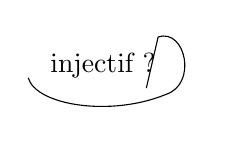
\begin{tikzpicture}[baseline=(n.base)]\node(n) at (0,0){injectif ?};\draw (0.7,0.37) .. controls (1.05,0.48) and (1.2,-0.23) .. (0.8,-0.36) .. controls (0.1,-0.65) and (-0.85,-0.5) .. (-0.95,-0.15);\draw (0.7,0.37)--(0.55,-0.28);\end{tikzpicture}}
\diagram{\begin{tikzcd}
\operatorname{Diff}^{(i)}_+(E,P)\arrow[r]&\operatorname{Hom}\mathrm{add}(\operatorname{Ker}d_E^1,P)
\end{tikzcd}}
\margin{l'image est \unsure{appelé|appelée}: faisceau des op. diff. de $\operatorname{Ker}d_E^1$ dans $P$}

Pour $i$ fixé, le $P$ ``universel'' pour les op. diff à coeff constants (d'ordre $\leq i$) sur $E$ est
\[
P^{(i)}(E)/\underline{O}_S.\delta_i^{\unsure{E}}(E),
\]
où
\[
\delta_i:E\longrightarrow P^i(E)
\]
est défini par la stratification.

3) Supposons maintenant donné un sous-Module $N$ de $E$, on s'intéresse aux hom ``différentiels'' $\operatorname{Ker}d_E^1\to P$ qui s'annulent sur $d_E^0N$, qui correspondent donc aux op. diff. $E\unsure{\mathbin{-}|\to}P$, à coeff. cts, et qui s'annulent sur $N$, donc aux op. diff. $M=E/N\unsure{\mathbin{-}|\to}P$ qui \deleted{sont ``\unsure{formels}''} deviennent à coeff. cts sur $E$. Ils correspondent \inserted{(pour l'ordre $\leq i$),} aux hom linéaires
\[
P^i(M)\longrightarrow P
\]
qui s'annulent sur $\rho_iE$; où
\[
\rho_i:E\unsure{\mathbin{-}|\to}P^i(M)
\]
\margin{231}
